\documentclass[12pt,letter]{article}
\usepackage[moduleName={Mini Boss}]{KautenjaDSP}
\begin{document}
\titlePage{img/Logo}{img/Module}{img/KautenjaDSP}

% -------------------
% MARK: Overview
% -------------------

\section{Overview}

Mini Boss is an emulation and re-envisioning of the Yamaha YM2612 audio processing unit from the Sega Mega Drive and Sega Genesis. Mini Boss provides the key functionality of \textit{a single operator} from the Yamaha YM2612, in addition to some hacks, omissions, and re-envisioned features, namely,
\begin{itemize}
  \item \textbf{16-bit Audio:} It's 8 bits better than the previous generation of chips! This is marketing! We're actually lying though -- the YM2612 produced a \textit{14-bit} stream, and so does BossFight. You're not getting those 2 bits back; go cry about it.
  \item \textbf{Single Operator FM Synthesis:} Full control over the parameters including envelopes, multipliers, rate scalings, tunings, gates, and internal LFO modulation.
  \item \textbf{Feedback:} Feedback into the operator one for interesting timbres or total wave destruction and noise.
  \item \textbf{Looping Envelopes:} Transform the one-shot envelope generator into a looping AD envelope.
  \item \textbf{Low-Frequency Oscillator:} A shared low-frequency sine oscillator controls amplitude modulation and frequency modulation of each operator.
  \item \textbf{Mono Output:} The original YM2612 was stereo, but only because it had six channels of synthesis. Mini Boss is a monophonic voice so there is no built-in stereo processing.
\end{itemize}

% -------------------
% MARK: Panel Layout
% -------------------

\clearpage
\section{Panel Layout}

\begin{figure}[!htp]
\centering
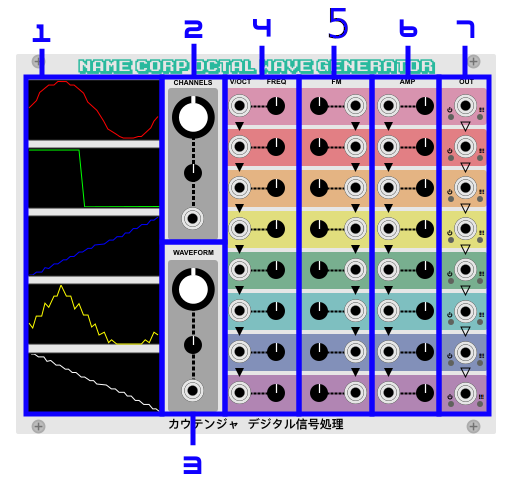
\includegraphics[width=\maxwidth{\textwidth}]{img/Interface}
\end{figure}

\subsection{Envelope Generator}

The envelope generator section provides control over the envelope generator parameters for each of the four operators on the module. Figure~\ref{fig:envelope-generator} depicts the stages in the envelope generator, where
\begin{itemize}
 \item \textbf{Total Level (\texttt{TL})} is the highest amplitude of the envelope generator. A change of one unit is about $0.75dB$;
 \item \textbf{Attack Rate (\texttt{AR})} is the angle of initial amplitude increase. This can be made very steep if desired. The problem with slow attack rates is that if the notes are short, the release (called \texttt{key off}) occurs before the note has reached a reasonable level;
 \item \textbf{Decay Rate (\texttt{D1R})} is the angle of initial amplitude decrease from the highest point in the envelope generator;
 \item \textbf{Total Level 1 (\texttt{T1L}):} The amplitude where the second decay stage starts;
 \item \textbf{Sustain Rate (\texttt{D2R})} is the angle of secondary amplitude decrease. This will continue indefinitely unless \texttt{key off} occurs; and
 \item \textbf{Release Rate (\texttt{RR})} is the final angle of amplitude decrease, after \texttt{key off}.
\end{itemize}

\begin{figure}[!htp]
\centering
\caption{An illustration of the stages in the envelope generator.}
\label{fig:envelope-generator}
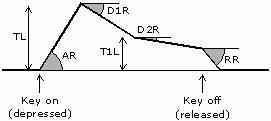
\includegraphics[width=\maxwidth{\textwidth}]{img/envelope}
\end{figure}

The \textbf{Rate Scale} parameter controls the amount of key-scaling that occurs for the envelope generator parameters $\in [0, 3]$, i.e., the degree to which envelopes become shorter as frequencies become higher. For example, high pitched notes on a piano fade much more quickly than the low pitched notes.

The \textbf{Loop} switch causes the envelope generator to enter a looping LFO mode when pointing up. When pointing down, the envelope generator is triggered by gate signals to the \textbf{GATE} port. The envelope generator can be re-triggered (i.e., triggered during a sustained note) using the \textbf{TRIG} port.

\subsection{Operator Control}

The operator control section provides control over the synthesis parameters of the operator, namely,

\begin{itemize}
 \item \textbf{Frequency} is the frequency offset for the operator. For standard FM sounds, all operators should be tuned to harmonically related frequencies. Individual operators with different frequencies is a special mode of the 3rd voice on the Yamaha YM2612 that can produce some weird and bizarre sounds;
 \item \textbf{LFO} is the rate of the internal low frequency oscillator $\in [0, 7]$ with frequency values mapped by Table~\ref{tab:lfo-frequencies}. The LFO is used for both amplitude and frequency modulation of the individual oscillators. When an input is patched to the \textbf{LFO} input, LFO frequencies can be selected in increments of $1V$;%
  \begin{table}[!htp]
  \centering
  \caption{Frequencies of the low-frequency oscillator.}
  \label{tab:lfo-frequencies}
  \begin{tabular}{|l|c|c|c|c|c|c|c|c|}
  \hline
  \bfseries Knob Position    & 0      & 1      & 2      & 3      & 4      & 5      & 6      & 7      \\
  \hline
  \bfseries Frequency ($Hz$) & $3.98$ & $5.56$ & $6.02$ & $6.37$ & $6.88$ & $9.63$ & $48.1$ & $72.2$ \\
  \hline
  \end{tabular}
  \end{table}
 \item \textbf{LFO Frequency Modulation} determines the amount of frequency modulation applied to the operator by the global LFO $\in [0, 7]$;
 \item \textbf{LFO Amplitude Modulation} determines the amount of amplitude modulation applied to the operator by the global LFO $\in [0, 3]$;
 \item \textbf{FM} polarizes and attenuates inputs to the \textbf{FM} port;
 \item \textbf{Multiplier} is an integer multiplier for the frequency of the operator. MUL ranges from $0$ to $15$, and multiplies the overall frequency, with the exception that $0$ results in multiplication by $\frac{1}{2}$;
 \item \textbf{Feedback} controls the amount of feedback for operator 1 $\in [0, 7]$. When an input is patched to the \textbf{FB} input, feedback levels can be selected in increments of $1V$; and
 \item \textbf{Volume} controls the output volume level from the synthesizer as an unsigned 7-bit multiplier.
\end{itemize}

\subsection{Envelope Generator Ports}

Each envelope generator parameter has an associated input port. The CV to each port is quantized uniformly from $[-8, 8]V$ continuous voltage to the discrete range of the associated parameter. Control voltages are indicated by the LED lights on the slider for the associated parameter. Positive (negative) voltages result in a green (red) light that increases in brightness as the voltage increases in magnitude.

\subsection{Voice Ports}

\begin{itemize}
 \item \textbf{GATE} input goes high at $2V$ and triggers the envelope generator on the operator. Figure~\ref{fig:envelope-generator} illustrates how the envelope generator interprets \texttt{key on} and \texttt{key off} events in the gate signal;
 \item \textbf{RTRG} input goes high at $2V$ and re-triggers the envelope generator on the operator if the gate is high;
 \item \textbf{VOCT} input provides exponential control for the oscillator's frequency offset from the base frequency determined by the \textbf{Frequency} knob;
 \item \textbf{FM} input allows for an external frequency modulation signal to be applied to the operator in addition to the feedback;
 \item \textbf{VOL} input controls the volume level output from the module. When an input is patched to the port, the \textbf{VOL} knob acts as an attenuator for the signal on the port; and
 \item \textbf{OUT} provides the monophonic output from the synthesizer $\in[-5,5]V$.
\end{itemize}

% -------------------
% MARK: Data Sheet
% -------------------

\clearpage
\section{Data Sheet}

\begin{table}[!htp]
\begin{tabular}{|l|l|}
\hline
Type             & Oscillator / Synth voice \\
\hline
Size             & 16 HP Eurorack           \\
\hline
Depth            & NA                       \\
\hline
Power            & NA                       \\ % 2 x 5 Eurorack
\hline
$+12V$ draw (mA) & 0 mA                     \\
\hline
$-12V$ draw (mA) & 0 mA                     \\
\hline
$+5V$ draw (mA)  & 0 mA                     \\
\hline
\end{tabular}
\end{table}

% -------------------
% MARK: References
% -------------------

\clearpage
\renewcommand\refname{References}
\nocite{*}
\bibliographystyle{apalike}
\bibliography{references}

\end{document}
